\documentclass[../dissertation.tex]{subfiles}
\title{}

\begin{document}
\maketitle

\chapter{Empirical Food Webs and the Parasitic Niche}

\begin{abstract}
While previous studies have investigated the occurrence of parasites in food
webs, none to the author's knowledge were dedicated solely to the
differentiation of free-living from parasitic taxa; this difference was always
taken to be self-evident. We question that premise and ask in what ways
parasites differ from free-livers apart from the relative size of their
resources. We study the parasite and free-living carnivore communities in a set
of highly resolved food webs using ecologically familiar and unfamiliar
properties of nodes within a network. We hope that going beyond the simple in
and out degree of nodes will help to show new patterns and encourage the use of
more network theoretic measures in other areas of food web research. We also
investigate the resilience of observed patterns to decreases in trophic
resolution.
\end{abstract}

\section{Introduction}

The structure of empirical food webs - contrary to the random network of interactions
studied by Mays 40 years ago - display predictable patterns of interactions.
It has been shown that the body size relationships between predator and prey,
while varying between habitat categories and metabolic classes, consistently
show that predators eat prey that are smaller than themselves
\cite{Brose2006a}. Body-size relationships, then, may play a role in defining
Mays's infamous ``devious strategies.'' 

These trends, when identified, conveniently omitted parasites from their
analyses; this is largely because historical food web data omitted parasites
taxa entirely \cite{Marcogliese1997}. The extent to which observed patterns of
body-sizes are robust to the inclusion of parasites has not been rigorously
analyzed; it should be clear, however, that parasites represent an
energetically important and diverse community of species. The inclusion of
these taxa in future analyses can only refine past results. Understanding the
roles that parasites play in the topology food webs can help to understand
their larger place in an ecosystem.

Fortunately the last fifteen years have seen the construction of several
species-rich food webs that contain well-resolved communities of parasites.
These food webs have been the subject of numerous studies exploring, for
example, the effect of parasites on the fit of theoretical web models, their
robustness to species removal, and the connection between biomass production,
trophic level, and metabolic rates \cite{Dunne2013, Lafferty2012,
Hechinger2011b}. This study extends previous work by attempting to elucidate
unique features of parasitic niches in these food webs with the aim of
generating a set of rules that identify parasites strictly by their local
topological properties within a food web.

We also investigate the effect of trophic resolution on the ability of
community and node properties to distinguish free liver from parasite. It has
been shown that a well-resolved food web is robust to modest decreases in
trophic resolution \cite{Martinez1991}. Untangling the role of variable 
resolution in food webs remains an important question \cite{Martinez1999}.

\section{Data} 
Following \cite{Dunne2013}, we analyzed 6 food webs containing well-resolved
parasite communities and more than 100 functionally distinct ``trophic
species'' each of which contain all taxa that share the exact same set of
predators (\ref{tab:foodWebSummary}).

%We analyzed 6 speciose food webs with well-resolved parasite
%communities. See table \ref{tab:foodWebSummary} for a summary of the basic
%structural properties in each of the six webs after trophic aggregation; more
%detailed descriptions can be found in the literature \cite{Dunne2013}. 

All six food webs represent coastal ecosystems. Three are located on the pacific
coast of southern California and Mexico \cite{Hechinger2011a}; two are located
on the north sea \cite{Thieltges2011,Zander2011}; one is located in a large
natural harbor in New Zealand \cite{Mouritsen2011}. 


 \begin{table}
    \centering
    \begin{tabular}{r l l l l l l }
        \toprule
        Full Name               &Code       &$S$    &$C$    &$S_p$  &$S_f$  &Reference\\
        \midrule 
        Bahia Falsa San Quintin &BSQ        &185    &0.083  &49
                                &127&\cite{Hechinger2011a}\\
        Carpinteria Salt Marsh  &CSM        &154    &0.084  &56     &88
                                &\cite{Hechinger2011a}\\
        Estero de Punta Banda   &EPB        &147    &0.079  &68     &70
                                &\cite{Hechinger2011a}\\
        Flensburg Fjord         &FF         &141    &0.090  &41     &94 &\cite{Zander2011}\\
        Otago Harbor            &OH         &117    &0.077  &17     &96&\cite{Mouritsen2011}\\
        Sylt Tidal Basin        &STB        &109    &0.071  &29     &74&\cite{Thieltges2011}\\
        \bottomrule
    \end{tabular}
    \caption{This table shows the size (species richness, $S$) and complexity
        (connectance, $C$) of the 6 trophic webs studied \cite{Dunne2013}. $S_p$ is the richness of
    parasitic species and $S_f$ is the richness of free-living species.
    \label{tab:foodWebSummary}}
\end{table}


\section{Methods} 

\subsection{Constructing Trophic Webs} We first constructed trophic webs from
each of 6 of 7 food webs described by \cite{Dunne2013}. We excluded the food
web of the Ythan Estuary because it ignored all consumption of parasites. Table
1.2 summarizes how links were originally classified in the raw data and how we
classified them for our construction of the food webs. We distinguished two
different link types: (1) free-living consumption and (2) parasitism. We
classified a species as a parasite if it was the consumer node in a parasitism
link; all other consumers were classified as free-livers. The empirical data
also distinguished life stages of many but not all species. We addressed this
inconsistency by aggregating all the life stages of a species into a single
node; we then aggregated these species-level nodes with identical consumer and
resource sets into trophic webs to create webs identical to those in
\cite{Dunne2013}. 

\begin{table}
    \centering
    \begin{tabular}{r l l}
        \toprule
        Link Type                                   & Parasitic?    & Prevalence\\
        \midrule
        Predation                                   & No            &29.3\%\\%
%        Social Predation                            & N/A           &0\%\\
        Micropredation                              & No            &1.4\%\\%
        Parasitic Castration                        & Yes           &0.7\%\\%
        Pathogen Infection                          & Yes           &0.1\%\\%
        Macroparasitism                             & Yes           &10.9\%\\%
%        Pollination                                 & N/A           &0\%\\
        Parasitoid Infection                        & N/A           &$<$0.1\%\\%
        Commensalism                                & N/A           &$<$0.1\%\\%
        Trophic Transmission*                       & N/A           &11.1\%\\%
%        TT Parasitic Castration                     & N/A           &0\%\\
%        TT Pathogen Infection                       & N/A           &0\%\\
%        TT Commensalism                             & N/A           &0\%\\
        Trophically Transmitted Parasitism          & Yes           &3.9\%\\%
        Concurrent Predation on Symbionts*          & N/A           &29.6\%\\%
        Predation on free-living non-feeding stages & No            &7.7\%\\%
        Predation on commensal non-feeding stages   & No            &0.1\%\\%
        Detritivory                                 & No            &1.3\%\\%
        Parasite Intraguild Antagonism              & Yes           &3.0\%\\%
%        Symbiotic Mutualism                         & No            &0\%\\
%        Facultative Micropredation                  & No            &0\%\\
        \bottomrule
    \end{tabular}
    \caption{This table describes how link types in the empirical data
        were used to construct food webs. A ``Yes'' under the ``Parasitic?''
        column indicates that we defined the consumer in such links to be a
        parasite; an ``N/A'' in the same column indicates that we excluded that
        link type from our analysis. Link types marked by * denote concomittant
        links; we omit these from our analysis because they are well predicted
        by a simple structural algorithm as they arise solely from the
        interactions of two other organisms. See \cite{Hechinger2011a} for complete
        descriptions of all link types.
    \label{tab:foodWebLinks}}
\end{table}

We also tracked species classes in the trophic aggregation stage; a node in the
trophic web was labeled as either Invertebrate, Ectotherm Vertebrate,
Endotherm, or basal. This was done using the taxonomic classes of the
individual species nodes; these four types of species never occupied the same
topological niche so there was no ambiguity in our final classification of each
trophic species. We also tracked the body size of each trophic node; the
resulting body size of an aggregated trophic node is the geometric mean of the
body sizes of each species comprising the node. Only the webs compiled in
\cite{Hechinger2011a} had body size data.

\subsection{Properties of Parasites} We calculated both common and more novel properties of
nodes in an attempt to find a structural fingerprint of parasitism. The
properties calculated include traditional local properties of ecological
interest (vulnerability, generality, and trophic level, represented by $v_i$,
$g_i$, and $T_i$, respectively) and network theoretic properties not commonly
found in ecological studies.

\subsubsection{Clustering Coefficients}
Parasites violate conventional body size relationships where larger predators
typically consume smaller prey. This may lead to unusual topological
neighborhoods where parasite consumers and resources interact more or less
frequently than that which occurs in the neighborhoods of more conventional
predators and prey. In order to explore this possibility, we calculated four
different directed clustering coefficients following \cite{Fagiolo2007}.
The clustering coefficient of a network is generally considered to be the
probability that two nodes that are linked to a third node are also linked to
each other. While typically calculated at the whole web level, it can also be
calculated for an individual node as the probability that two of that node's
neighbors are themselves linked together. Such coefficients are conceptually
straightforward int he case of non-directed links; directional links such as
feeding relationships complicate the calculation of such coefficients.


In undirected networks, the clustering coefficient of a node is the fraction of
possible links between all of its neighbors. We calculated this clustering
coefficient by ignoring link direction within our data. However, this approach
can be unsatisfactory because different patterns of directed links between a
node and its neighbors are likely to be important, especially in the case of
food webs. Table \ref{tab:triangles} provides a more technical summary of our 4
clustering coefficients.

Note that the definitions in table \ref{tab:triangles} require the existence of
two links in the appropriate orientation for the clustering coefficient to be
defined for a given node. This is particularly troublesome when averaging to
determine a global web property as the common solution of defining the
clustering for nodes with one or zero links to be zero can skew the average if
there are many nodes with only one link (see \cite{Kaiser2008}). When
calculating the clustering of a community of species, instead of averaging
individual coefficients, we consider the fraction of links for each individual
in the entire community simultaneously; thus, for a community of $\mathcal{I}$
nodes, the community level clustering coefficient for $\mathcal{I}$ is found by
summing the numerator and denominator of the equations in table
\ref{tab:triangles} over $i\in\mathcal{I}$. Clustering coefficients for
individual species with just one link are set to zero.
\tikzset{littleNode/.style={circle,draw=black,inner sep =1pt}}
\tikzset{curvyEdge/.style={bend right = 10}}
\definecolor{gray70}{gray}{.7}
\newcommand\makeTriangleNodes[3]{%
            \draw (0,0) node [littleNode,fill=gray70] (#1) {\tiny$_i$};
            \draw (1,0) node [littleNode] (#2) {\tiny$_j$};
            \draw (.5,.866) node [littleNode] (#3) {\tiny$_k$};}
 \begin{table}
     \centering
     \begin{tabular}{m{0.3\textwidth} m{0.3\textwidth} m{0.3\textwidth}}
        \toprule
        Formula    &Triangles Counted&Interpretation\\\midrule
        \multicolumn{3}{l}{Consumer Clustering}\\\cmidrule(r){1-1}
        $\gamma_i^{c} = \frac{(A^2A^\top)_{ii}}{v_i(v_i-1)}$  
        &\begin{tikzpicture}%Cyclic Triangle
            \makeTriangleNodes{i}{j}{k}
            \path [->,>=stealth]
            (i) edge  node [right] {} (j)
            (j) edge[gray70]  node [right] {} (k)
            (i) edge  node [right] {} (k);
        \end{tikzpicture}\hspace{.1in}%
        \begin{tikzpicture}%Cyclic Triangle
            \makeTriangleNodes{i}{j}{k}
            \path [->,>=stealth]
            (i) edge node [right] {} (k)
            (k) edge [gray70]  node [right] {} (j)
            (i) edge  node [right] {} (j);
        \end{tikzpicture}&
        Fraction of possible links between consumers.\\
        \multicolumn{3}{l}{Resource Clustering}\\\cmidrule(r){1-1}
        $\gamma_i^{r}= \frac{(A^\top A^2)_{ii}}{g_i(g_i-1)}$
        &\begin{tikzpicture}%Sink 1
            \makeTriangleNodes{i}{j}{k}
            \path [->,>=stealth]
            (j) edge  node [right] {} (i)
            (j) edge[gray70]  node [right] {} (k)
            (k) edge  node [right] {} (i);
        \end{tikzpicture}\hspace{.1in}%
        \begin{tikzpicture}%Sink 2
            \makeTriangleNodes{i}{j}{k}
            \path [->,>=stealth]
            (j) edge node [right] {} (i)
            (k) edge [gray70]  node [right] {} (j)
            (k) edge  node [right] {} (i);
        \end{tikzpicture}&
        Fraction of possible links between resources.\\
        \multicolumn{3}{l}{Resource Consumer Clustering}\\\cmidrule(r){1-1}
        $\gamma_i^{rc}=\frac{(AA^\top A)_{ii}}{g_iv_i-(A^2)_{ii}}$            
        &\begin{tikzpicture}%Cyclic Triangle
            \makeTriangleNodes{i}{j}{k}
            \path [->,>=stealth]
            (i) edge  node [right] {} (j)
            (k) edge[gray70]  node [left] {} (j)
            (k) edge   node [right] {} (i);
        \end{tikzpicture}\hspace{.1in}%
        \begin{tikzpicture}%Cyclic Triangle
            \makeTriangleNodes{i}{j}{k}
            \path [->,>=stealth]
            (i) edge node [right] {} (k)
            (j) edge [gray70]  node [right] {} (k)
            (j) edge  node [right] {} (i);
        \end{tikzpicture}&
        Fraction of possible links from resources to consumers.\\
        \multicolumn{3}{l}{Consumer Resource Clustering}\\\cmidrule(r){1-1}
        $\gamma_i^{cr}= \frac{(A^3)_{ii}}{g_iv_i-(A^2)_{ii}}$
        &\begin{tikzpicture}%Cyclic Triangle
            \makeTriangleNodes{i}{j}{k}
            \path [->,>=stealth]
            (i) edge node [right] {} (j)
            (j) edge [gray70]  node [right] {} (k)
            (k) edge  node [right] {} (i);
        \end{tikzpicture}\hspace{.1in}%
        \begin{tikzpicture}%Cyclic Triangle
            \makeTriangleNodes{i}{j}{k}
            \path [->,>=stealth]
            (i) edge node [right] {} (k)
            (k) edge [gray70]  node [right] {} (j)
            (j) edge  node [right] {} (i);
        \end{tikzpicture}&
        Fraction of possible links from consumers to resources.\\
        \bottomrule
    \end{tabular}
    \caption{This table summarizes the four types of clustering coefficients as
        found in \cite{Fagiolo2007}. We have renamed the clustering
        coefficients to better reflect the ecological interpretation. All
        formulae are for node $i$; $A$ is the adjacency matrix without
        cannibalism, $(M)_{ii}$ is the $(i,i)$-th entry of a matrix $M$, $g_i$
        is the (non-normalized) generality of node $i$, and $v_i$ is the
        (non-normalized) vulnerability of node $i$.  The clustering coefficient
        is the fraction of times the gray links appear given the existence of
        the black links in each sub-graph. 
    \label{tab:triangles}}
\end{table}

\subsubsection{Betweenness centralities} Betweenness centrality is a measure of
how often a particular node appears in shortest paths between each other pair
of nodes. This measure was developed in the context of information flow through
social networks; nodes with a high betweenness are likely to be gatekeepers
between highly connected components. The original measure for a node $v$, as developed in
\cite{Freeman1977,Anthonisse1971} is

\begin{equation} 
    C_B(v) = \sum_{s\neq v\neq t\in V}\frac{\sigma_{st}(v)}{\sigma_{st}}
\label{eq:BetweennessCentrality} 
\end{equation}

where $\sigma_{st}(v)$ is the number of shortest paths between node $s$ and $t$
that pass through $v$, and $\sigma_{st}$ is the total number of shortest paths
between nodes $s$ and $t$.

We offer a slight refinement of betweenness centrality by only counting
shortest paths between a basal species and a consumer species. The ecological
betweenness centrality, $C_{EB}$ of a node $v$, is given by:

\begin{equation} 
    C_{EB}(v) = \sum_{s\in\text{bas},t\in\text{con},t\neq v}\frac{\sigma_{ij}(v)}{\sigma_{ij}}
\label{eq:EcologicalBetweennessCentrality} 
\end{equation}
%
where $\sigma_{ij}$ and $\sigma_{ij}(v)$ are as in
\ref{eq:BetweennessCentrality}; basal and top species have $C_{EB}(i)=1$ and
$C_EB(i) = 0$, respectively. We believe this may be of greater ecological
significance as the shortest path to a basal is likely to be much more
energetically important for a species than the shortest path between two
species at similar trophic levels.

\subsubsection{Mean Generality of Consumers} This property is the average
normalized generality of all the consumers of a particular node. This aims to
measure the importance of a resource in the diet of its consumers. If
$\mathcal{C}_i$ is the set of consumers of $i$ and $g_j$ is the generality of
node $j$, then the mean generality of consumers of node $i$, $g_c(i)$ is given
by

\begin{equation} 
    g_c(i) = \frac{1}{|\mathcal{C}_i|}\sum_{j\in\mathcal{C}(i)}g_j
\label{eq:MeanGeneralityConsumers} 
\end{equation}

If a node $i$ has no consumers, we set $g_c(i)=0$. 


\subsubsection{Mean Vulnerability of Resources} This property is the average
normalized vulnerability of all the resources of a particular node. This aims
to measure the impact of a node on its resources. If $\mathcal{R}_i$ is the
set of resources of $i$ and $v_j$ is the vulnerability of node $j$, then the
mean vulnerability of resources of node $i$, $v_r(i)$ is given by

\begin{equation} 
    v_r(i) = \frac{1}{|\mathcal{R}_i|}\sum_{j\in\mathcal{R}(i)}v_j
\label{eq:MeanVulnerabilityResources}  
\end{equation}

If a node $i$ has no resources, we set $v_r(i)=0$.

\newcommand\FR{\mathit{FR}} 

\subsubsection{FlowRank} The PageRank measure achieved fame as one of the
metrics behind the popular Google search engine; webpages have a high PageRank
if webpages with high PageRank link to them, accounting for both the quantity
of links and the PageRank of each source node.  We follow \cite{Allesina2009b}
in a modification of the PageRank algorithm to create an eigenvalue-based
centrality measure suitable for food webs, which we call here FlowRank. The
idea behind FlowRank is that nodes should be "important" (i.e. have a high
FlowRank) if they are resources for important nodes. Note that the FlowRank
"importance" flows backwards along the food web links, that is, a node's
importance derives from its consumers (who the node points to), not its resources
(who points to the node). See \cite{Allesina2009b} for a full discussion of the
measure. In what follows, we denote the FlowRank of a node $i$ by
$\lambda_i$.

\subsubsection{Additional Concerns} The above measures can be highly dependent
on network size and complexity. To alleviate this issue, we normalize all of
the above metrics by dividing by the mean value among all consumers. This
scaling was chosen over a $z$-score standardization since many of the variables
studied are defined to be non-negative with a special meaning attached to zero,
which we wished to preserve. We then compare parasitic averages to carnivore
averages to account for the absence of parasites of basal species (for example,
no herbivorous insects were sampled in any of the webs) in all webs
tested.

\subsection{Agglomeration of Webs} We were also interested in how food web
resolution affected the above measures of centrality; aggregating trophically
similar species may result in a clearer structural signature of parasites. For
each of the 6 empirical webs, we used the unweighted pair group method with
arithmetic mean (UPGMA, \cite{Sokal1958}) with the Jaccard distance to group
similar nodes as in \cite{Martinez1991}. The Jaccard Distance,
\cite{Jaccard1908} is calculated as 

\begin{equation} 
    d_J(s,t) = 1-\frac{|\mathcal{N}(s)\cap \mathcal{N}(t)|}{|\mathcal{N}(s)\cup \mathcal{N}(t)|}
\label{eq:JaccardDistance} 
\end{equation} 

where $\mathcal{N}(v)$ is the set of all neighbors (i.e. all consumers and all
resources) of node $v$. We define the distance between two clusters of nodes using
average linkage clustering: for two clusters $\mathcal{A}$ and $\mathcal{B}$,
define $d_J(\mathcal{A},\mathcal{B})$ as

\begin{equation} 
    d_J(\mathcal{A},\mathcal{B}) = \frac{1}{|\mathcal{A}|\cdot|\mathcal{B}|}\sum_{s\in\mathcal{A}}\sum_{t\in\mathcal{B}}d_J(s,t)
\label{eq:averageLinkage} 
\end{equation}

The result of the clustering algorithm was a sequence of clusters of species;
in order to define a web at each level of aggregation, we also needed to define
feeding relationships between the clusters. We used the "maximum linkage
criterion" as defined in \cite{Martinez1991}. The six webs studied here had
much lower connectances than the Little Rock Lake food web, so more stringent
linkage criteria (i.e. the "mean linkage criterion") quickly resulted in
disconnected webs. For each food web defined along the clustering sequence, we calculated the
aforementioned nodal and global properties. 

\subsubsection{Breaking Ties} The sequence of clusters resulting from
agglomerative clustering algorithms are non-deterministic in the presence of
ties in the distance between pairs of clusters. At each step in the clustering
algorithm, we first identified all potential mergers between clusters. We then
label the smaller cluster the \textit{satellite} and the larger cluster the
\textit{sink} for each merger; if the two clusters for a given merger were the
same size, each cluster had equal probability of being assigned as the sink.
After identifying the satellite and the sink, we model the merger of two
clusters as the satellite being subsumed into the sink. Given a set of
potential mergers, we merge the smallest sinks first; ties between smallest
sinks were broken by choosing the merger with the smaller satellite; ties in
both sink and satellite size were broken at random. When a satellite merges
into a sink, it is ineligible for any further mergers. The sinks, however,
remain eligible for further mergers until they are subsumed into a larger sink.
We used the above procedure to encourage a more even distribution of nodes
among clusters. 

To account for stochasticity in the hierarchical clustering model, we ran 100
replicates of the clustering procedure for each web and averaged the results;
the coefficient of variation for all properties was under 0.001 suggesting that
the properties calculated are robust to small variations in the clustering
sequence. In what follows we report the results of a single clustering
procedure in the interest of simplicity.


\subsection{Parasite Classification} We constructed a binary classification
tree at each clustering level. At each level of species abundance, we used the
local properties described above of all carnivorous free livers and all
parasites in all available webs to train and test a classification tree, with
80\% of the nodes used to train each model and 20\% of the nodes used to
estimate the misclassification rate of all species and of parasites
specifically. We also analyzed the relative importance of each metric on all
classification trees. All trees were constructed using \verb|fitctree| in
MATLAB R2016b with a maximum of 4 splits. We chose a maximum of 4 splits to
avoid over-fitting and to ensure that the trees are easily comprehended.
Increasing the number of splits did not result in significant increases in the
error rates (results not shown).


\section{Results} 

\subsection{Body Sizes Relationships} We plotted the log-normalized body size
of consumers against the $\log_{10}$-normalized body size of resources raw food
webs including life stages (figure \ref{fig:bodySizeFig-a}) and trophic webs
(figure \ref{fig:bodySizeFig-b}). Links were colored according to the metabolic
type of the consumer; regression lines were calculated for each metabolic type
and $R^2$ values were calculated. The fitted slopes were fairly robust to
trophic aggregation except for those of parasites; the slope for parasites
decreased by a factor of ten after trophic aggregation, from $-0.40$ to
$-0.04$. The $R^2$ values also saw decreases; they decreased by factors of two
for invertebrates and ectotherm invertebrates, a marginal decrease for
endotherms, and to essentially zero for the parasites.

\begin{figure}
    \centering
    {%
        \phantomsubcaption{\label{fig:bodySizeFig-a}}%
        \phantomsubcaption{\label{fig:bodySizeFig-b}}%
    }%

        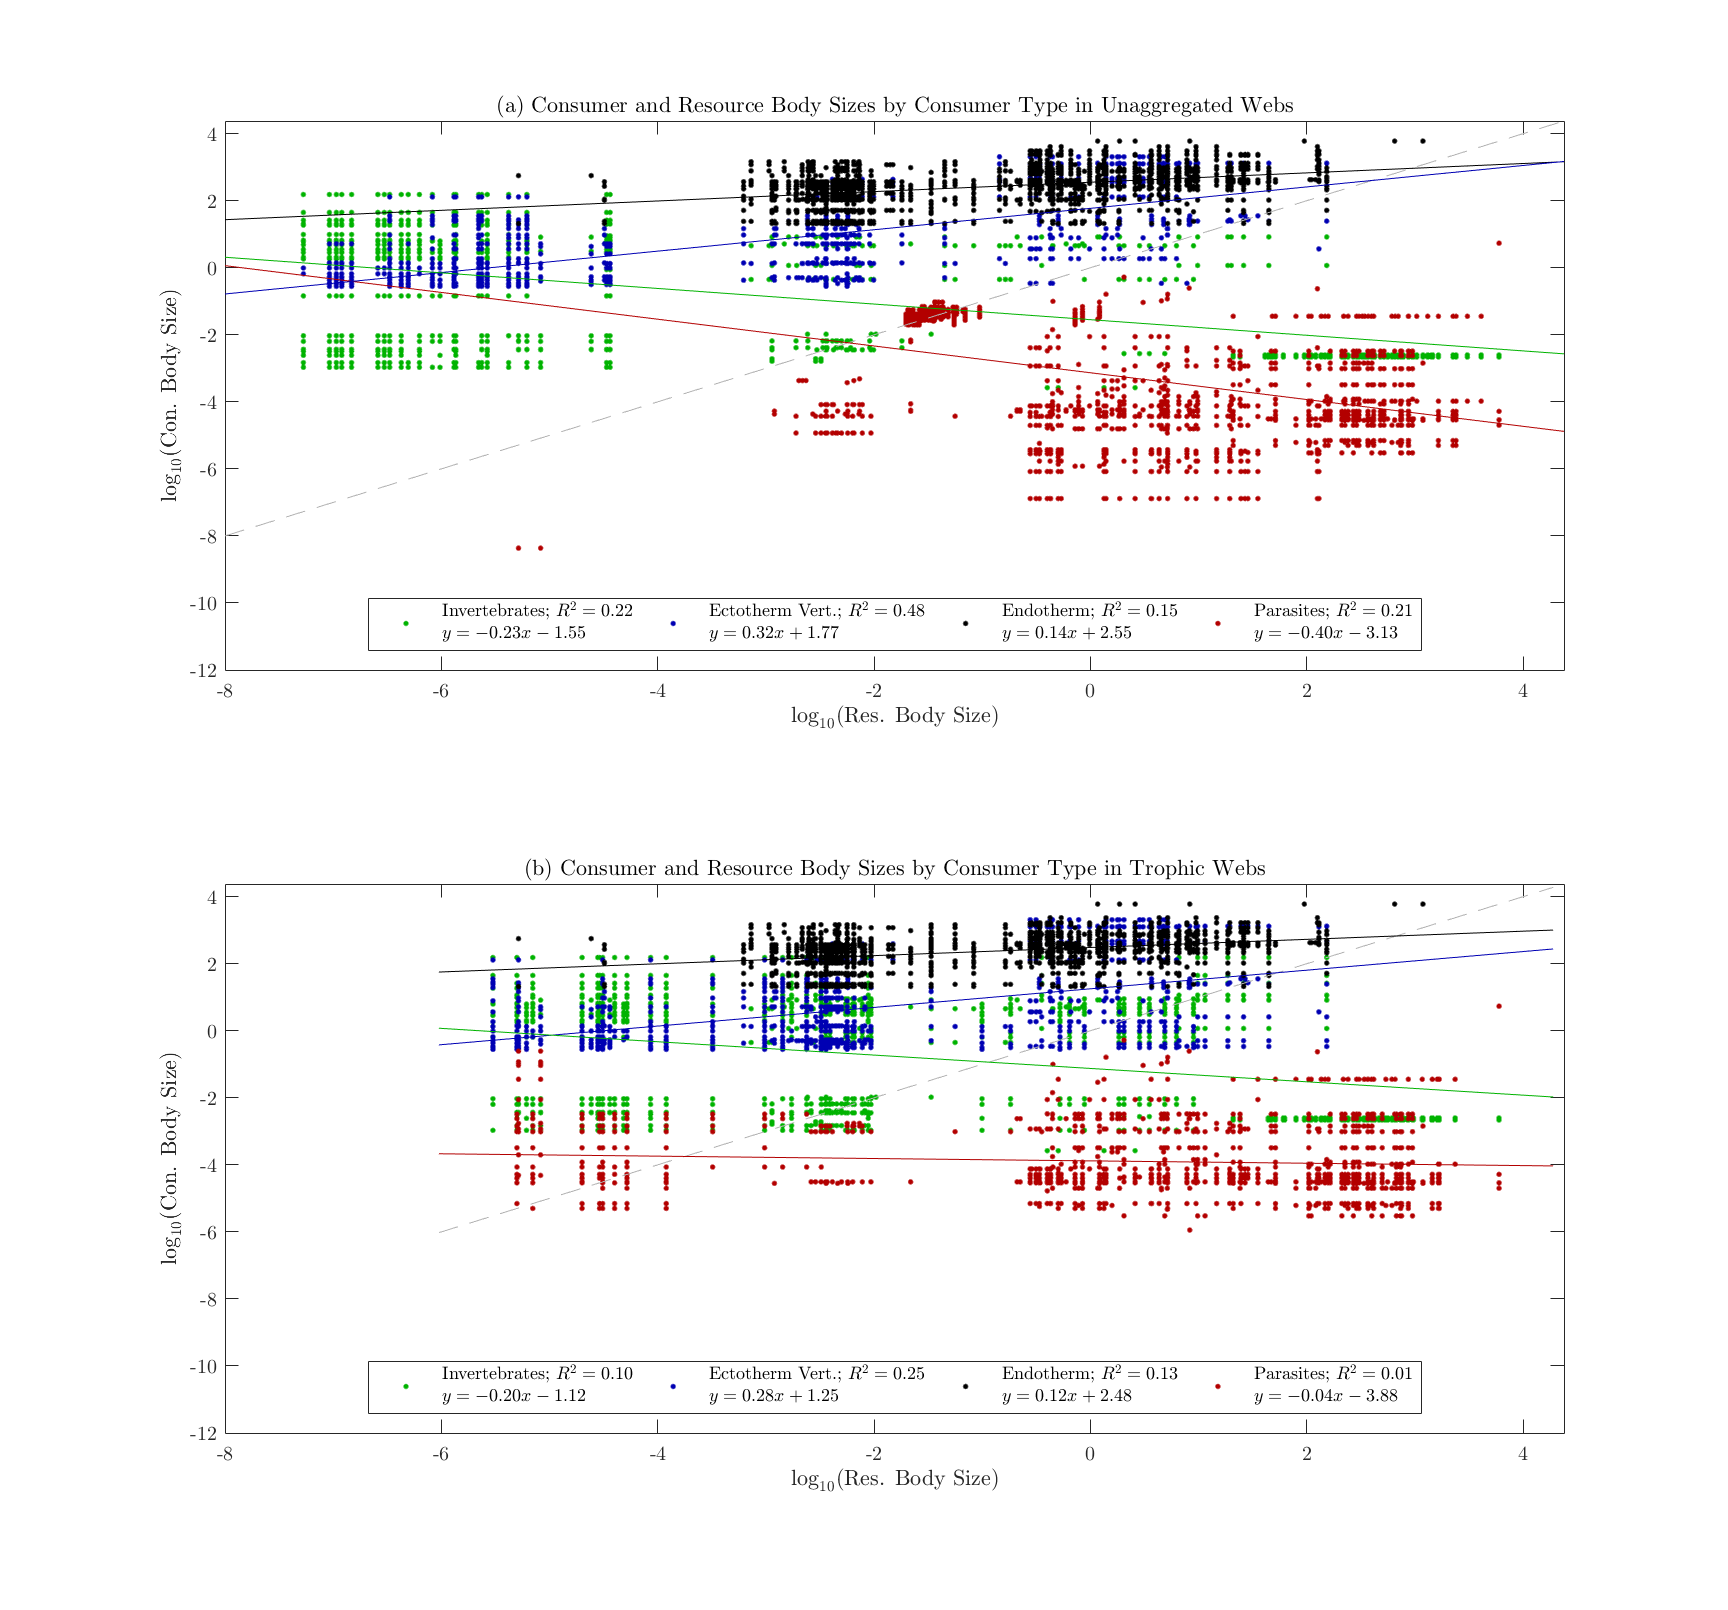
\includegraphics[width=\textwidth]{\DissertationDir/Chapter2/figures/bodySizes.png}
        \caption{This figure shows the $\log_{10}$-normalized body sizes for
            all links with body size data for both consumer and resource body
            size data in both the raw food web (figure \ref{fig:bodySizeFig-a})
            and the trophic food web (figure \ref{fig:bodySizeFig-b}). Links
            are colored according to the metabolic type of the consumer.
            Least-squares regression lines were calculated for each metabolic
            type and $R^2$ values were reported. The dashed line represents
            equality between consumer and resource body size.
        \label{fig:bodySizeFig}} 
\end{figure}

\subsection{Properties of Initial Trophic Webs} The parasite average plotted
against the carnivore average for each property for each empirical trophic web
is given in figure \ref{fig:initialNodalProperties}. Only one of the nine nodal
properties resulted in statistically significant differences between the
average value for parasites and free-livers when controlling the family-wise
error rate with the Bonferroni-Holm procedure at the 0.05 significance level.
See figure \ref{fig:initialNodalProperties} for a summary of the test results
on the initial trophic webs.

Despite the failure to reject 11 of the 12 null hypotheses, there was some
tentative evidence of systematic differences in the means of parasites and
carnivores in the trophic food webs prior to agglomeration. We found a
statistically significant difference between parasite and carnivore communities
in the community-level fraction of completed three-cycles (figure
\ref{fig:initialNodalProperties-i}).

Our statistical tests had a fairly low power due to both the number of
inferences (12) and the small sample size for each inference (6). As a result,
there were two properties with low $P$-values for which we were unable to
reject the null hypothesis; trophic level (figure
\ref{fig:initialNodalProperties-c}) and the community level fraction of realized
links between consumers (figure \ref{fig:initialNodalProperties-l}) both had
$P$-values less than 0.01 but were not low enough to warrant rejection by the
Bonferroni-Holm procedure.  

A further four properties had $P$-values below 0.05 but were considerably
larger than the cutoffs defined by the Bonferroni-Holm correction.
Vulnerability (figure \ref{fig:initialNodalProperties-a}), FlowRank (figure
\ref{fig:initialNodalProperties-d}), and the community level fractions of
realized links from resources to consumers and between resources (figures
\ref{fig:initialNodalProperties-j}, \ref{fig:initialNodalProperties-k}) also showed
some evidence of a difference between free-living and parasitic communities. 

Three properties showed a potential interaction with web size (marker size).
Vulnerability (figure \ref{fig:initialNodalProperties-a}) appeared to show a
slight increase for the carnivore average as web size increased while the
parasitic average remained relatively static. The community fraction of
realized links from resources to consumers (figure
\ref{fig:initialNodalProperties-j} also showed a potential relationship with
web size; as web size decreases we see a decrease in the fraction for the
parasite community while the fraction for the carnivore community remained
relatively static.  Finally, the fraction of links between consumers (figure
\ref{fig:initialNodalProperties-i}) also showed a decrease for parasites as web
size decreased and little change in the carnivore average.  However, given the
overall weakness of these trends and the small sample size of webs, we saw
little need to control for the effects of web size.

Two properties showed a potential interaction with web complexity (marker
color). FlowRank (figure \ref{fig:initialNodalProperties-d}) showed the
strongest interaction; as complexity increased, the parasitic FlowRank
decreased and the carnivore FlowRank increased. Vulnerability (figure
\ref{fig:initialNodalProperties-a}) also showed a potential relationship of
increasing carnivore average with increasing complexity while the parasite
average remained the same. Again, given the fairly weak nature of these
relationships and the fact that they occurred in only a sixth of the properties
meant that we saw little need to control for web complexity either.

\begin{sidewaysfigure}       
    \centering
    {%
        \phantomsubcaption{\label{fig:initialNodalProperties-a}}%
        \phantomsubcaption{\label{fig:initialNodalProperties-b}}%
        \phantomsubcaption{\label{fig:initialNodalProperties-c}}%
        \phantomsubcaption{\label{fig:initialNodalProperties-d}}%
        \phantomsubcaption{\label{fig:initialNodalProperties-e}}%
        \phantomsubcaption{\label{fig:initialNodalProperties-f}}%
        \phantomsubcaption{\label{fig:initialNodalProperties-g}}%
        \phantomsubcaption{\label{fig:initialNodalProperties-h}}%
        \phantomsubcaption{\label{fig:initialNodalProperties-i}}%
        \phantomsubcaption{\label{fig:initialNodalProperties-j}}%
        \phantomsubcaption{\label{fig:initialNodalProperties-k}}%
        \phantomsubcaption{\label{fig:initialNodalProperties-l}}%
    }% 
    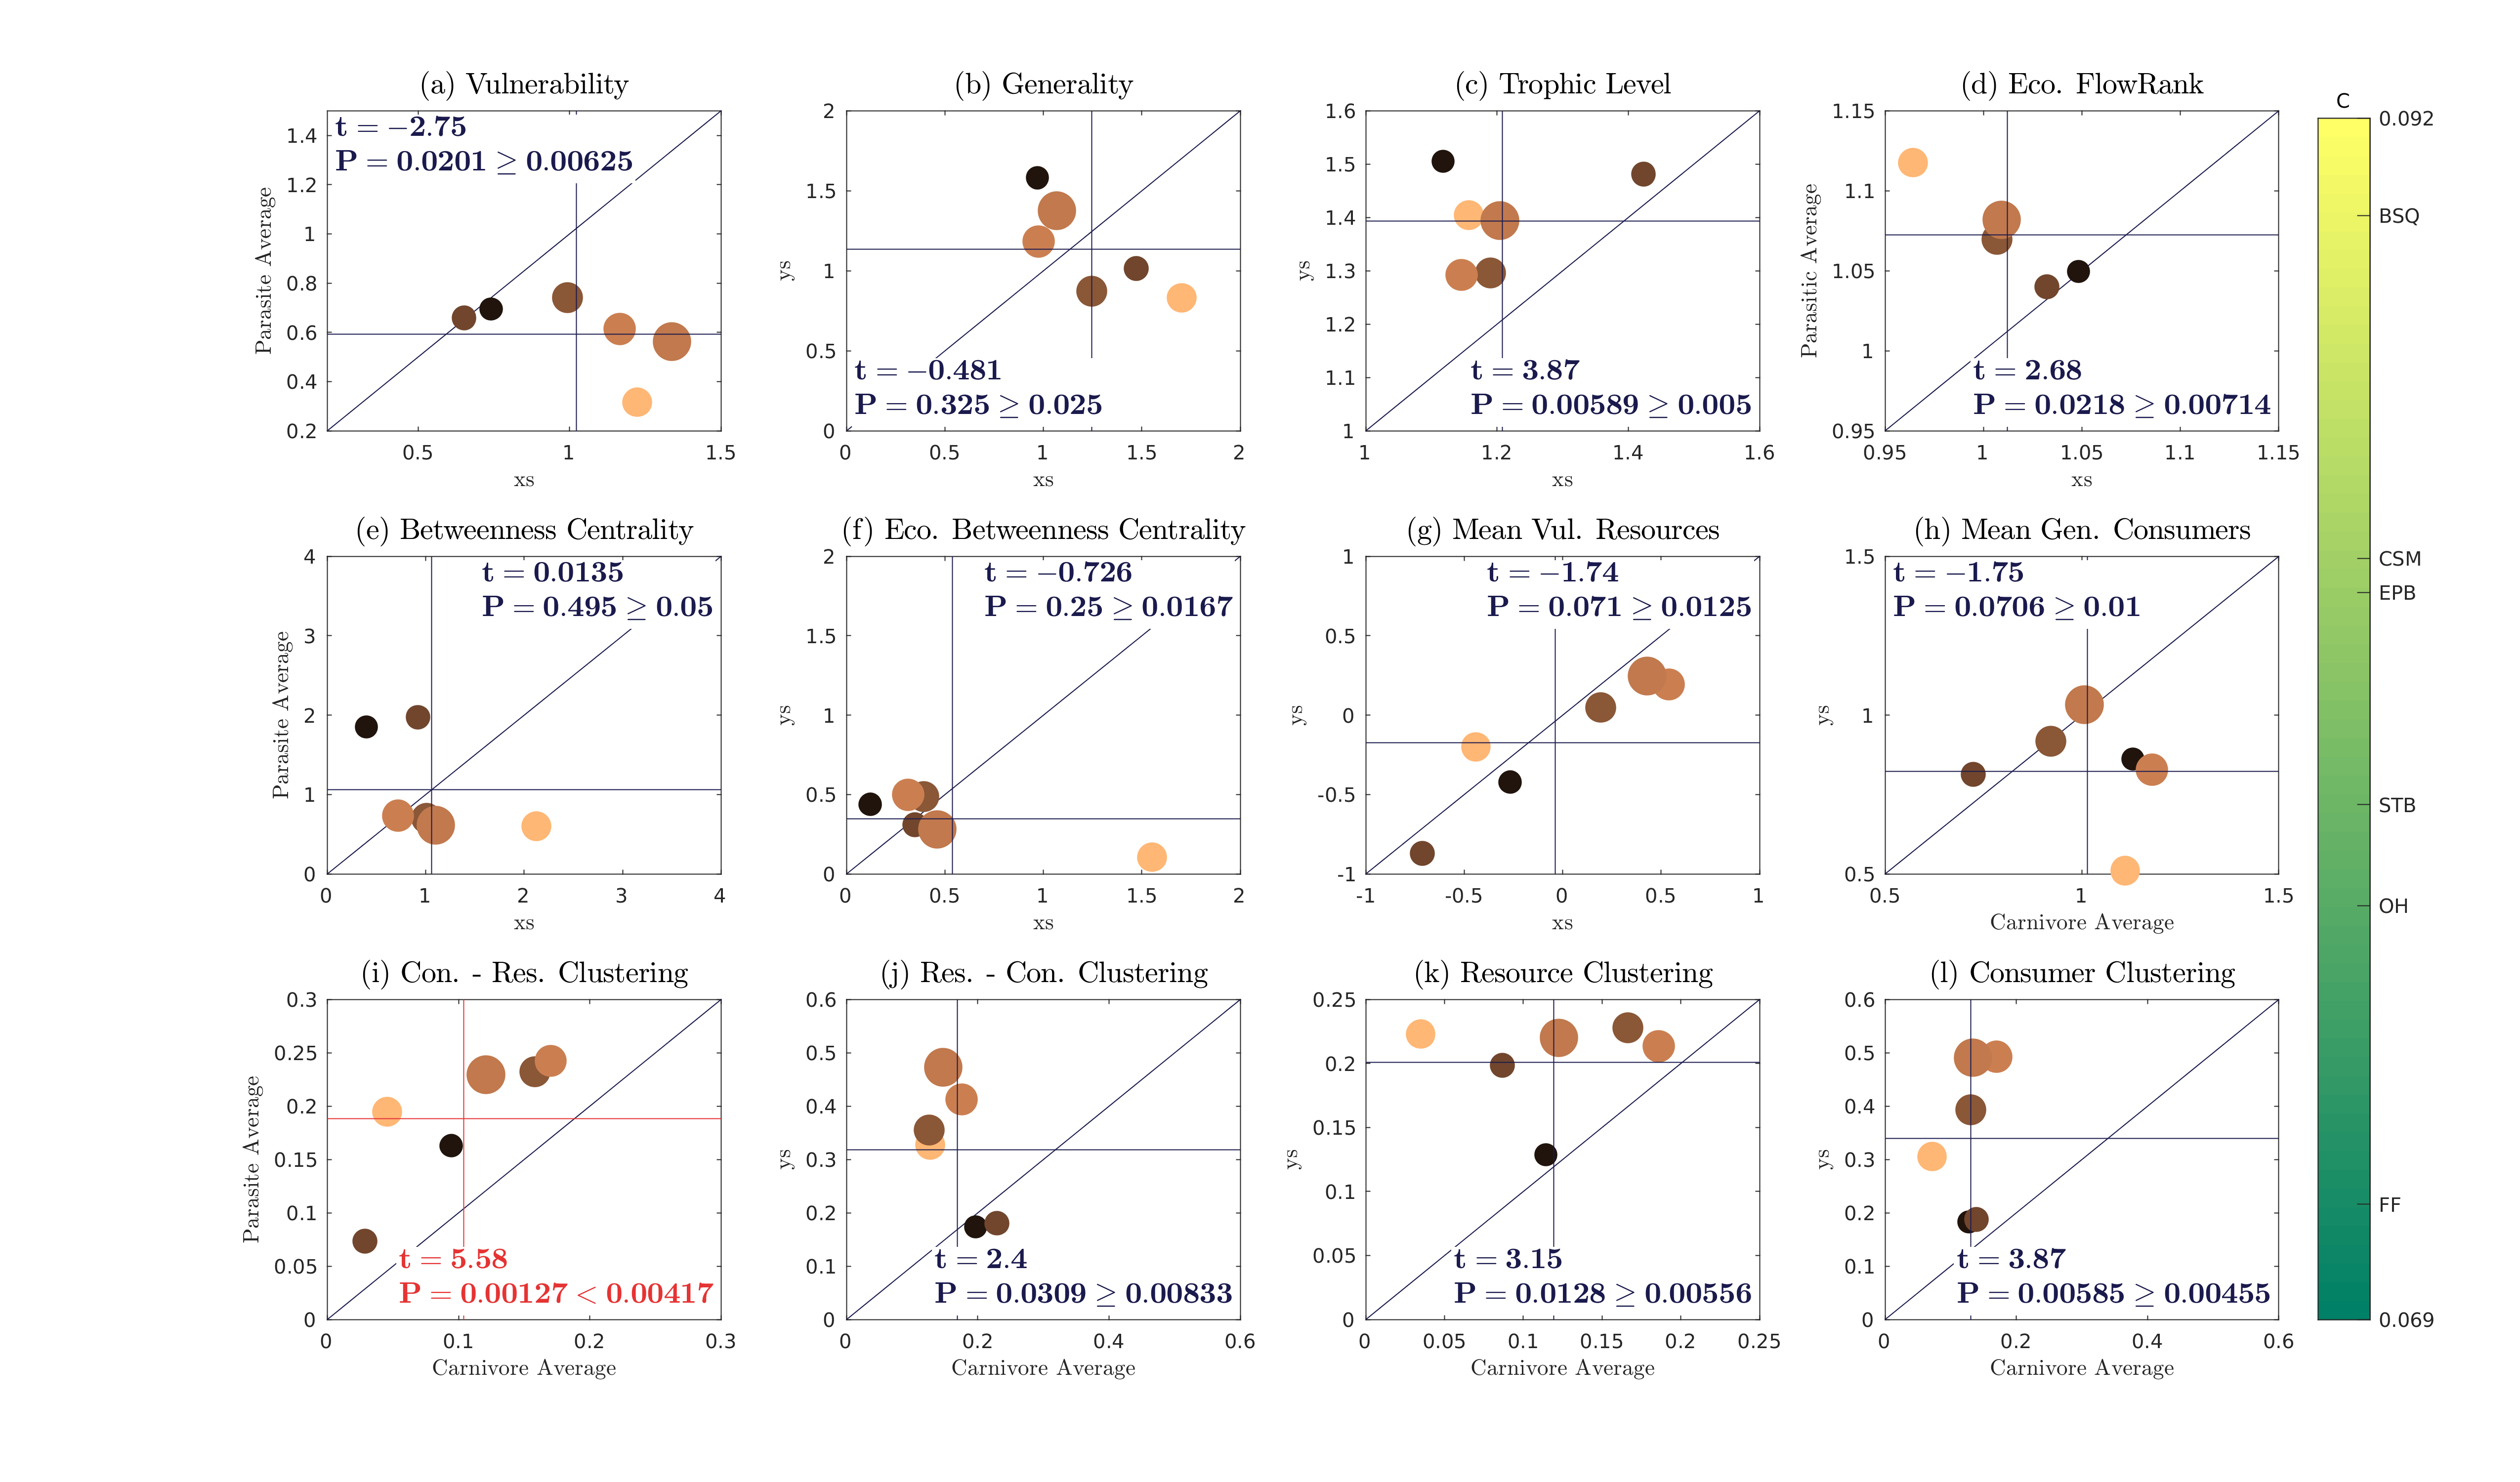
\includegraphics[width=\linewidth]{\DissertationDir/Chapter2/figures/initialPropsMaxLinkage.png}

    \caption{This figure shows the average value among parasites ($y$-axis) and
        free-livers ($x$-axis) for each property and each web. Dot size is
        proportional to the species abundance and colored according to the
        connectance of the corresponding web.  The average among the 6 webs for
        free-livers is denoted by the vertical line and for parasites by the
        horizontal line. The vertical and horizontal lines are colored red if
        the mean difference between the free-liver and parasitic value in each
        web is significantly different from zero. We performed two sided
        $t$-tests and controlled the family-wise error rate at $\alpha=0.05$
        using the Bonferroni-Holm procedure. We also report the corresponding
        $t$ statistics and $P$-values for the hypothesis tests. The diagonal
        line represents equality between free-livers and
        parasites.\label{fig:initialNodalProperties}}
\end{sidewaysfigure}

\subsection{Agglomerated Webs}

We calculated the average similarity within and between parasites, carnivores,
and free livers but not between carnivores and free livers (figure
\ref{fig:meanDistFig}). We omit the last comparison as carnivores are a subset
of the free livers. We used the clusters from the clustering sequences to
calculate these values, not the resulting food webs. While the ordering of the
mean distance within the groups was not consistent across all 6 webs, we do
observe that the mean distance between the groups is always higher than the
mean distance within, implying that species of the same class are much more
likely to merge with each other than with species in different classes. This
trend is not held for carnivores and free livers; this is not surprising as
carnivores are a subset of the free livers.

\begin{figure}
    {%
        \phantomsubcaption{\label{fig:meanDistFig-a}}%
        \phantomsubcaption{\label{fig:meanDistFig-b}}%
        \phantomsubcaption{\label{fig:meanDistFig-c}}%
        \phantomsubcaption{\label{fig:meanDistFig-d}}%
        \phantomsubcaption{\label{fig:meanDistFig-e}}%
        \phantomsubcaption{\label{fig:meanDistFig-f}}%
    }% 
    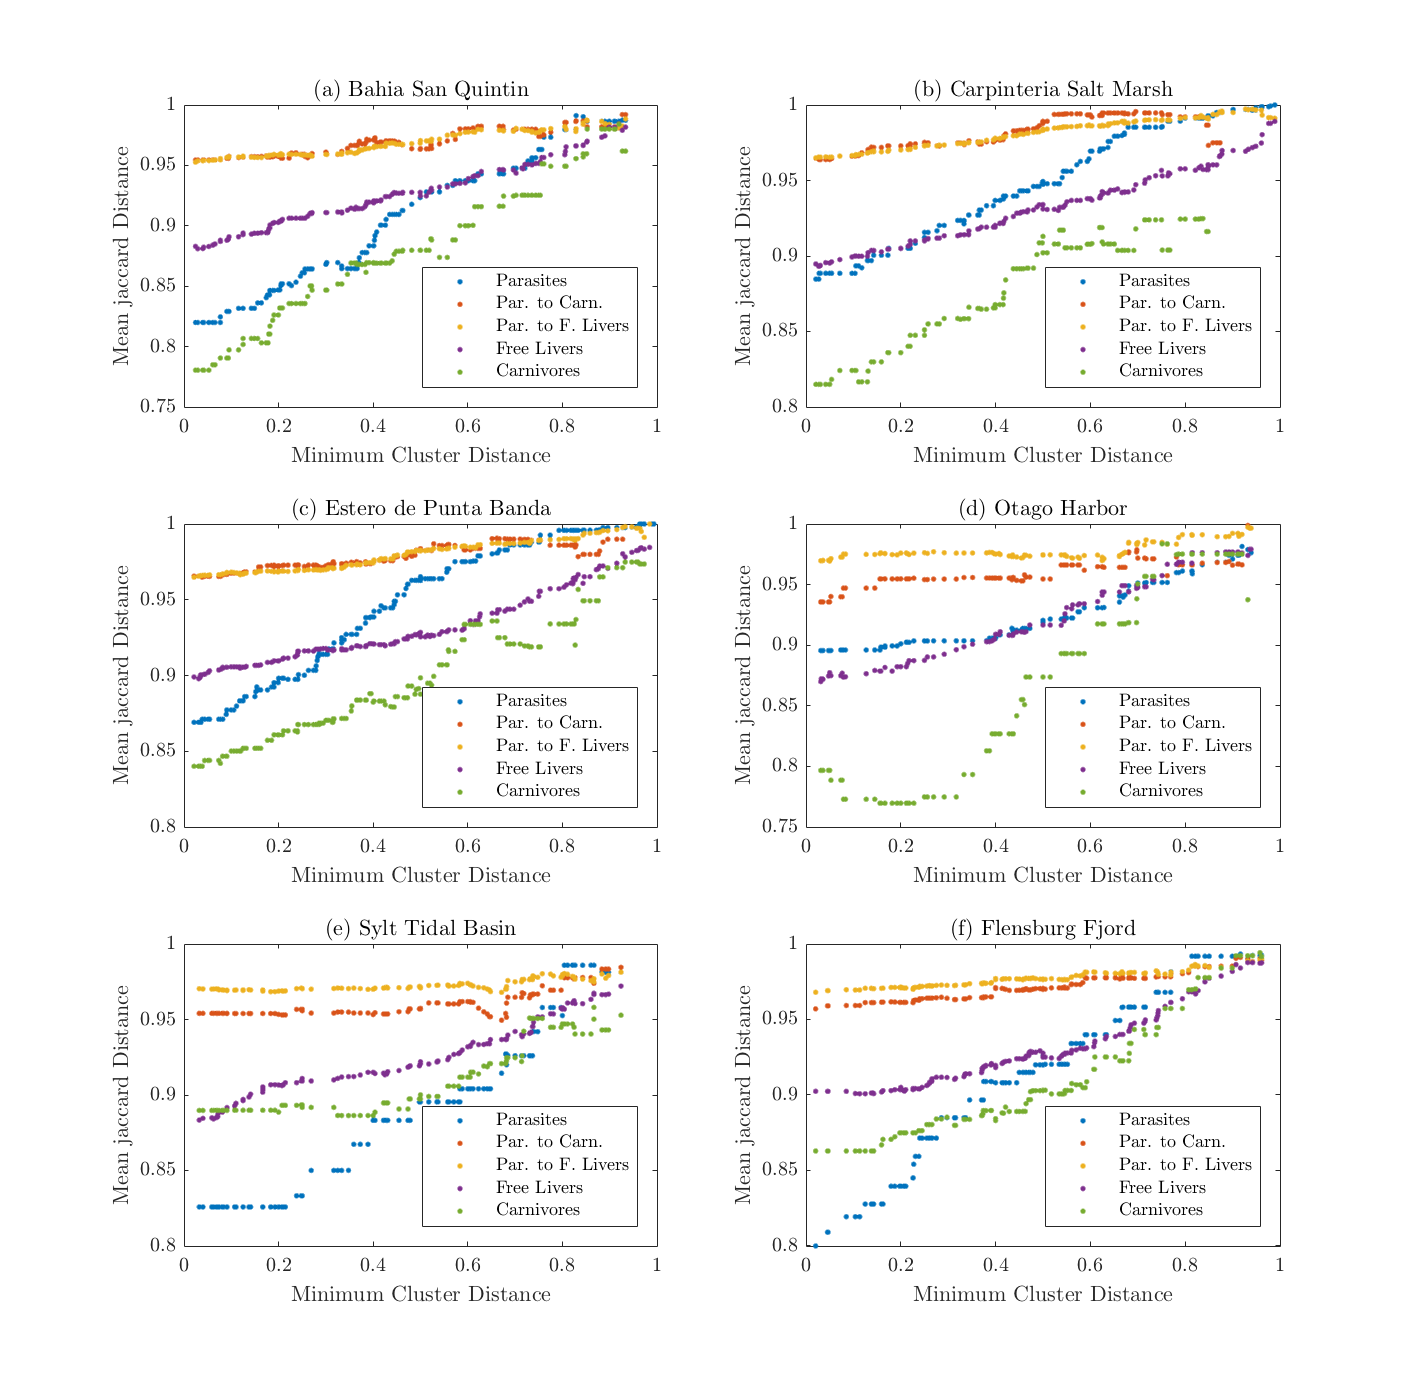
\includegraphics[width=\linewidth]{\DissertationDir/Chapter2/figures/meanClassDist.png}

    \caption{This figure shows the minimum distance between different type of
        species in the agglomeration sequence for each web. Noe that these
        are the mean Jaccard distances before links between species are formed
        in the food webs.
    \label{fig:initialNodalProperties}}

\end{figure}

We also calculated all properties at each clustering level. Figure
\ref{fig:allNodalProperties} shows the differences between the average values
of parasites and free livers for each web plotted against the minimum distance
between clusters. Very few properties showed that the difference between the parasite and
carnivore average was significantly different from zero; notice that at a
minimum cluster distance of 0 the analysis is identical to that in
figure \ref{fig:initialNodalProperties}. 

The difference in community level fraction of completed three cycles (figure
\ref{fig:allNodalPropertiesDistances-i}) continues to be significant up to a
minimum cluster distance of 0.7. We also see that the community level fraction
of realized links between consumers (figure
\ref{fig:allNodalPropertiesDistances-l}) is significant for clustering levels
from about 0.1 to 0.6. These two properties were the only ones that reliably
showed significant differences; however, many of the properties identified in
the previous section were consistent in the sign and magnitude of the
difference between parasitic and carnivore communities; only the community
level fraction of realized links from resources to consumers (figure
\ref{fig:allNodalPropertiesDistances-j}) and the community level of realized
links between resources (figure \ref{fig:allNodalPropertiesDistances-k})
reversed their initial trends. The failure to identify these as significant
differences may again be due to the small sample size and large family of tests
being conducted. Note that we only applied the Bonferroni-Holm correction at
each minimum cluster distance.


%\begin{figure}[t]       
%    {%
%        \phantomsubcaption{\label{fig:allNodalPropertiesLevels-a}}%
%        \phantomsubcaption{\label{fig:allNodalPropertiesLevels-b}}%
%        \phantomsubcaption{\label{fig:allNodalPropertiesLevels-c}}%
%        \phantomsubcaption{\label{fig:allNodalPropertiesLevels-d}}%
%        \phantomsubcaption{\label{fig:allNodalPropertiesLevels-e}}%
%        \phantomsubcaption{\label{fig:allNodalPropertiesLevels-f}}%
%        \phantomsubcaption{\label{fig:allNodalPropertiesLevels-g}}%
%        \phantomsubcaption{\label{fig:allNodalPropertiesLevels-h}}%
%        \phantomsubcaption{\label{fig:allNodalPropertiesLevels-i}}%
%        \phantomsubcaption{\label{fig:allNodalPropertiesLevels-j}}%
%        \phantomsubcaption{\label{fig:allNodalPropertiesLevels-k}}%
%        \phantomsubcaption{\label{fig:allNodalPropertiesLevels-l}}%
%    }% 
%    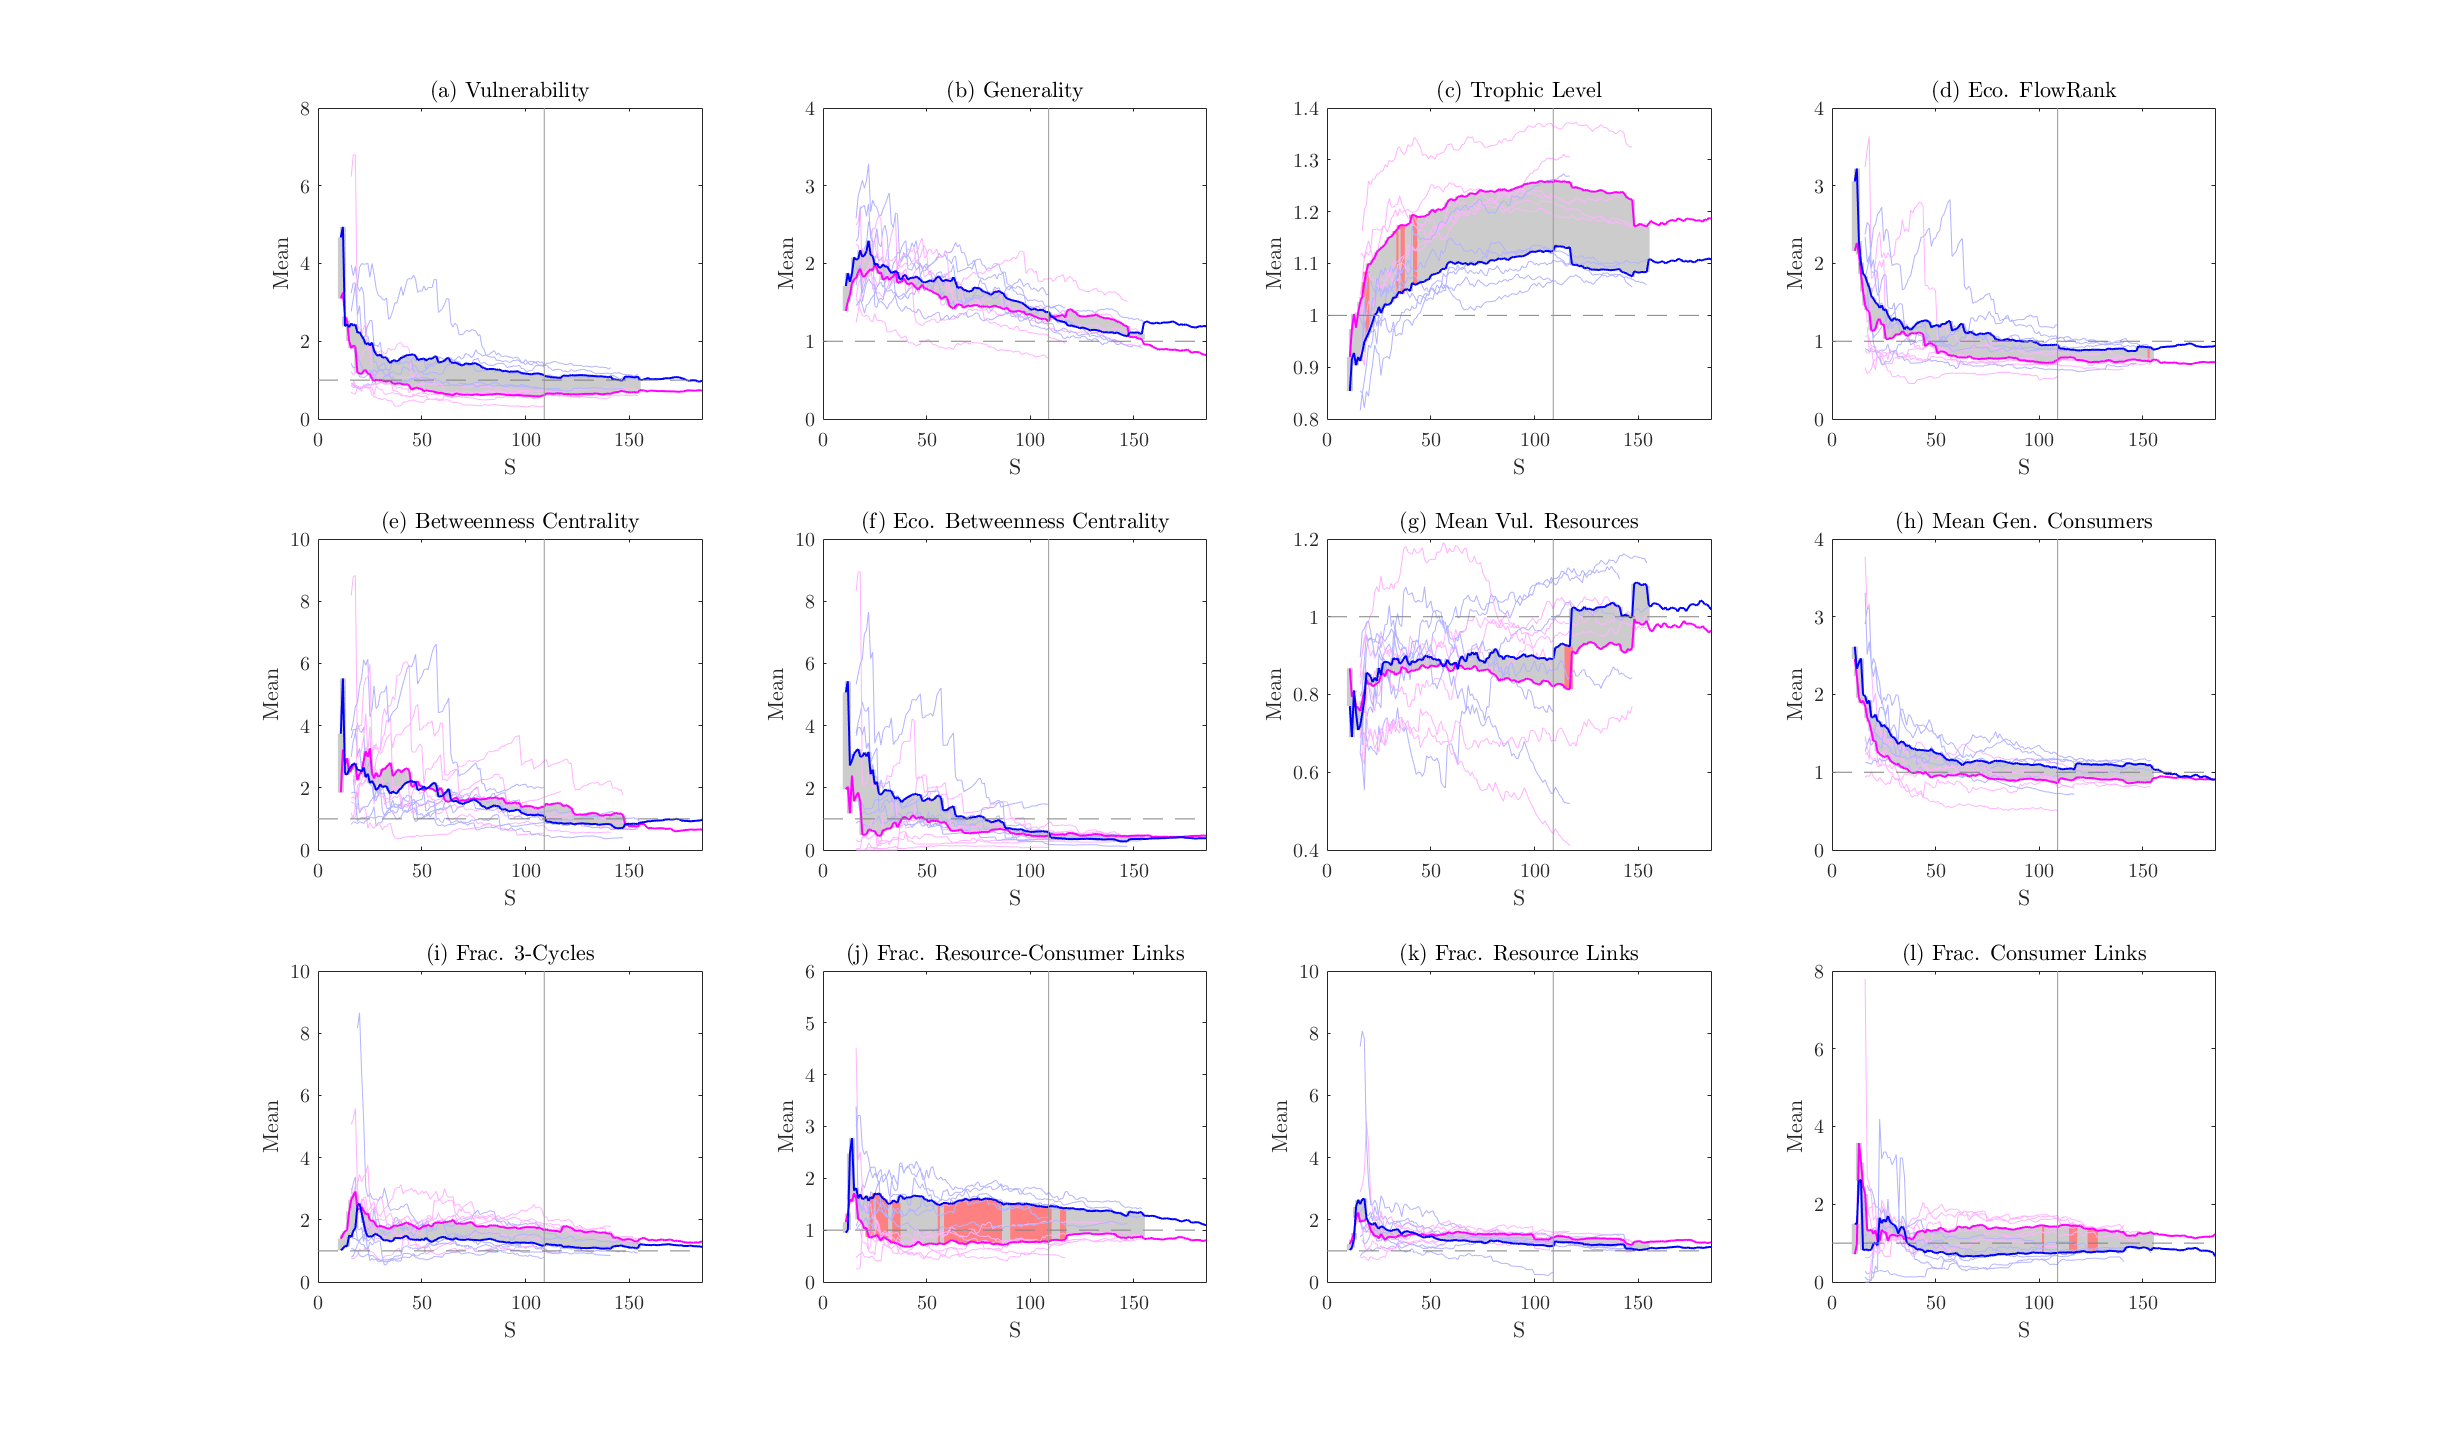
\includegraphics[width=\linewidth]{\DissertationDir/Chapter2/figures/allProps.png}
%    \caption{This figure shows the average across all 6 webs of the mean value
%        for each property for parasites (pink) and free-livers (blue). Red
%        shading between the two curves indicates clustering levels where the
%        mean of the difference between the free-liver average and the parasite
%        average is statistically significant. We conrolled the family-wise
%        error rate at $\alpha=0.05$ using the Bonferroni-Holm procedure at each
%        level of abundance. Note that above $S=154$ there was only one web so
%        that region was left unshaded to indicate that no test was performed.
%        The vertical line represents the point below which all webs were
%        used in the significance tests.
%        \label{fig:allNodalProperties}}
%\end{figure}

\begin{sidewaysfigure}       
    \centering 
    {%
        \phantomsubcaption{\label{fig:allNodalPropertiesDistances-a}}%
        \phantomsubcaption{\label{fig:allNodalPropertiesDistances-b}}%
        \phantomsubcaption{\label{fig:allNodalPropertiesDistances-c}}%
        \phantomsubcaption{\label{fig:allNodalPropertiesDistances-d}}%
        \phantomsubcaption{\label{fig:allNodalPropertiesDistances-e}}%
        \phantomsubcaption{\label{fig:allNodalPropertiesDistances-f}}%
        \phantomsubcaption{\label{fig:allNodalPropertiesDistances-g}}%
        \phantomsubcaption{\label{fig:allNodalPropertiesDistances-h}}%
        \phantomsubcaption{\label{fig:allNodalPropertiesDistances-i}}%
        \phantomsubcaption{\label{fig:allNodalPropertiesDistances-j}}%
        \phantomsubcaption{\label{fig:allNodalPropertiesDistances-k}}%
        \phantomsubcaption{\label{fig:allNodalPropertiesDistances-l}}%
    }% 
    \includegraphics[width=\linewidth]%
            {\DissertationDir/Chapter2/figures/allPropsDistMajority.png}
    \caption{This figure shows the differences between the carnivore average
        and parasite average in each web at each agglomeration level (thin gray
        lines) as well as the average of the 6 differences (thick blue line).
        Agglomeration levels with a difference between parasite and free-liver
        averages that was significantly different from zero are marked with a
        red line; others were marked with a gray line. Theses tests were
        corrected to control the family-wise error rate at each agllomeration
        level using the Bonferroni-Holm procedure. Agglomeration level was
        measured by the minimum distance between any two nodes in a clustered
        web.  Non-uniformity in this measure within and across webs meant that
        ensuring all 6 webs were averaged at required us to bin distances and
        average multiple agglomeration levels for each web before averaging
        across webs
    \label{fig:allNodalProperties}}
\end{sidewaysfigure}

\subsection{Classification of Parasites}

We analyzed the importance of the entire set of variables by training 100
classifiers with all predictors, with each predictor removed (figures
\ref{fig:initialClassResults-a}, \ref{fig:initialClassResults-c}) and with each
predictor in isolation (figures \ref{fig:initialClassResults-b},
\ref{fig:initialClassResults-d}). We measured overall classification error as the
fraction of the error in a random model.

We found that the classification error increased
the most when $\gamma^{c}$ was removed; this variable also had the least
increase in error from the full model when it was used in isolation and
resulted in fewer parasites misclassified than the full model. The removal of
any other predictor had little effect on the misclassification rates.

The mean generality of consumers was the next most effective variable when used
in isolation, as measured by the overall misclassification rate; however this
variable resulted in a much higher misclassification rate of parasites. The
rest of the variables had higher overall misclassification rates and all but
one had higher misclassification rates for parasites. The mean fraction of
completed three cycles resulted in fewer misclassified parasites than the full
model. Two of the variables, generality and mean vulnerability of prey, barely
beat the random classifier.

\begin{figure}
    \centering
    {%
        \phantomsubcaption{\label{fig:initialClassResults-a}}%
        \phantomsubcaption{\label{fig:initialClassResults-b}}%
        \phantomsubcaption{\label{fig:initialClassResults-c}}%
        \phantomsubcaption{\label{fig:initialClassResults-d}}%
    }%
        \includegraphics[width=\textwidth]%
            {\DissertationDir/Chapter2/figures/treeAnalysisc.png}
        \caption{This figure shows the importance of the twelve
            predictors for identifying parasites. Figures
            \ref{fig:initialClassResults-a} and \ref{fig:initialClassResults-c}
            show the performance of classifiers with one of the variables
            removed. Figures \ref{fig:initialClassResults-b} and
            \ref{fig:initialClassResults-d} show the results with one of the
            variables isolated. The $y$-axis in figures
            \ref{fig:initialClassResults-a} and \ref{fig:initialClassResults-b}
            represent the misclassification rate as a fraction of the error of
            the model that chooses an appropriate fraction of parasites
            uniformly at random; the exact value changes depending on the
            breakdown of the training set but has an expected value of 49.68\%. The
            dashed line in each figure represent the performance of a
            classifier with all 12 predictors; thus, the
            model including all variables has a misclassification rate of about
            15\%. Bar height is the average over 1000 replicates with different
            training/test splits. Error bars represent 95\% confidence
            intervals for the mean.
        \label{fig:initialClassResults}}
\end{figure}

We also calculated classification trees at all agglomeration levels up to a
minimum distance of 0.4. We first computed 1000 regression trees at each
agglomeration level with different splits between training and test data. At
each training level we recorded the 4 most frequently used predictors. We chose
to use only four because there are far fewer parasites and carnivores at the
higher levels of agglomeration; we then computed a further 100 webs at each
agglomeration level using only the identified most commonly occurring
predictors.  The results for those 8,100 classification trees are given in
figure \ref{fig:seqClassResults}. The overall error was relatively stable,
remaining between 0.27 and 0.37 across all agglomeration levels. Within this
range, there was considerable variability with no clear trend. The parasite
misclassification rate was also quite low, remaining between 0.06 and 0.13 for
the agglomeration levels calculated; this measure also showed a high degree of
variability.

The identity of two of the four most frequently used predictors was the same at
all agglomeration levels tested (figure \ref{fig:seqClassResults-b}). Trophic
level was commonly used in all but a few of the classification trees. FlowRank,
betweenness centrality, and mean generality of consumers were the next most
commonly used predictors; the rest were either never used or used just a few
times. Notice that the three most commonly used predictors corresponded to
variables that had small $P$-values in figure \ref{fig:initialNodalProperties}.

\begin{figure}
    \centering
    {%
        \phantomsubcaption{\label{fig:seqClassResults-a}}%
        \phantomsubcaption{\label{fig:seqClassResults-b}}%
    }%

        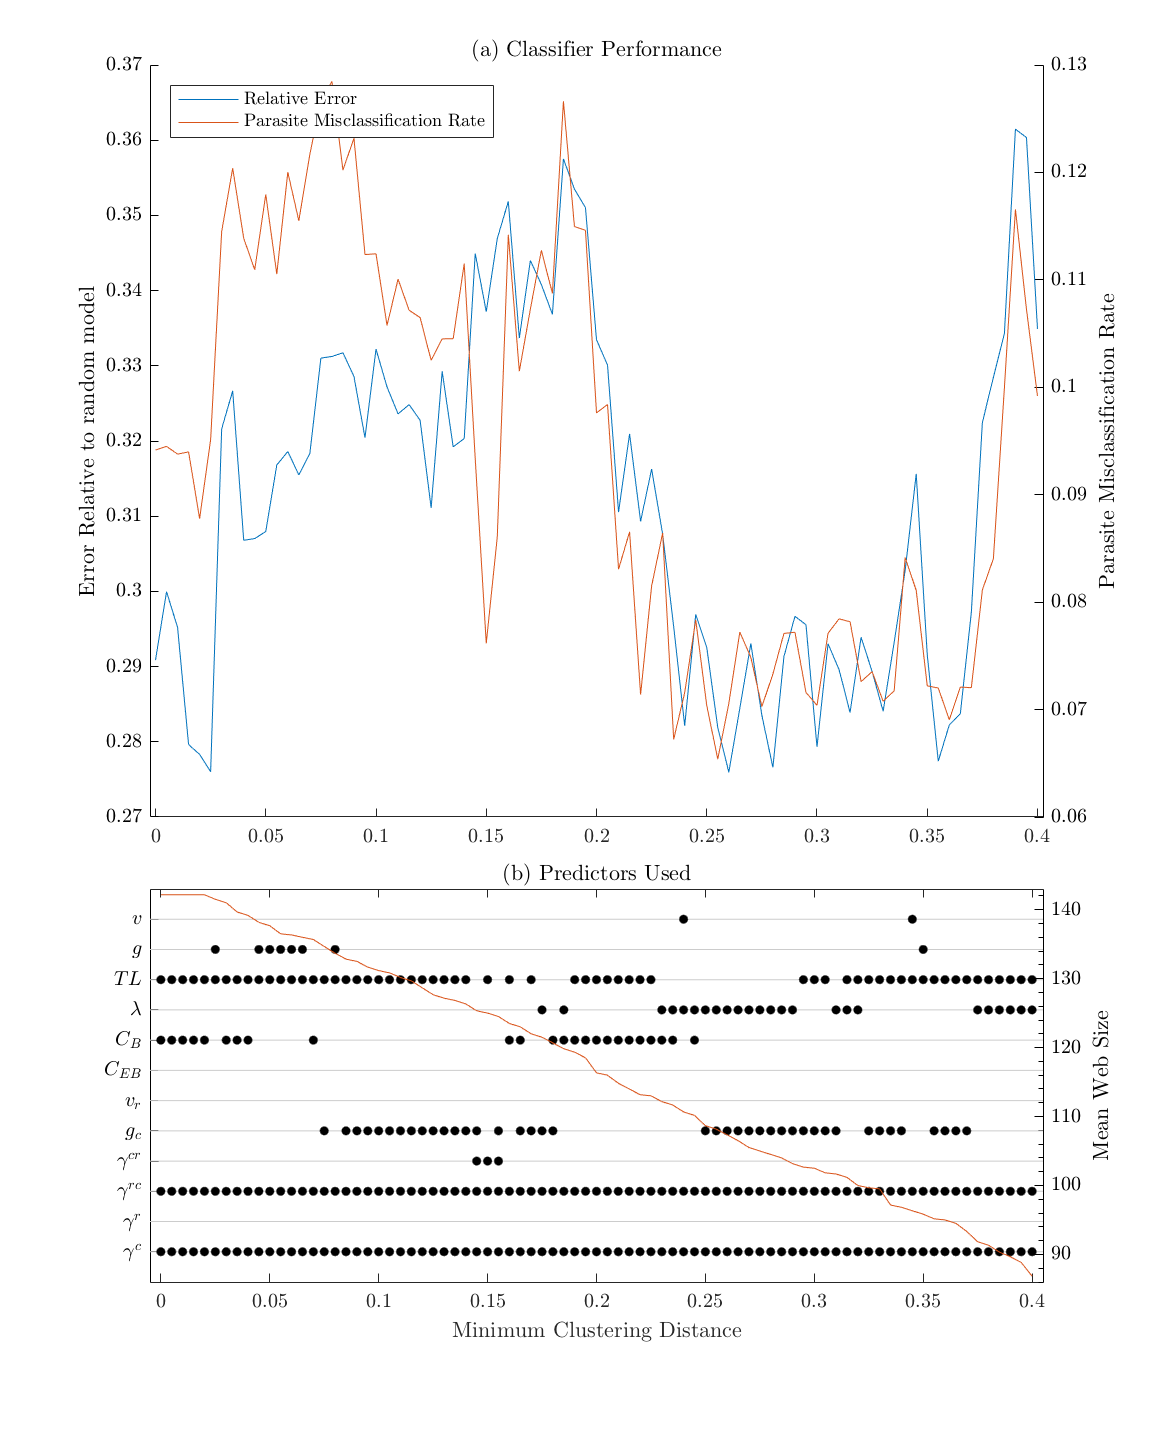
\includegraphics[width=0.7\textwidth]{\DissertationDir/Chapter2/figures/ParasiteAccMaxLinkage.png}
        \caption{This figure shows the average misclassification rate over 100
            replicates (figure \ref{fig:seqClassResults-a}) and the predictors
            used at each agglomeration level (figure
            \ref{fig:seqClassResults-b}). Figure \ref{fig:seqClassResults-b}
            also shows the relationship between cluster distance and average
            web size of all six webs at that clustering level.  
        \label{fig:seqClassResults}} 
\end{figure}

\section{Discussion} 

\subsubsection{Trophic Aggregation Complicates Trends in Body Size
Relationships} We found that trophically aggregating species and life stages
weakened observed trends in consumer-resource body size patterns. This effect
was most pronounced in parasites, where a significant cluster of links was
entirely lost. This effect was not confined to parasites as the predictive
power of the least-square regression line was significantly weakened in 3 of
the 4 metabolic types. 

This decrease in predictive power was likely caused by ambiguities in the
appropriate body size in aggregated nodes, especially when aggregating distinct
life stages that may have unique sets of resources, for example combining
parasitic life stages that are predators in a free-living life stage could
obscure interesting trends. This result is generally in line with results from
\cite{Gilljam2012}, which shows that computing body size ratios in interactions
between individuals resulted in much stronger patterns than when averaging body
sizes between species. 

\subsubsection{Distinguishing Parasitic and Carnivorous Communities} We found
that there were some fairly reliable ways to distinguish carnivore and parasite
communities. In the initial trophic webs, there were seven metrics with
$P$-values below 0.05. Six of those seven metrics had differences that were
robust to agglomeration, even up to minimum clustering distances of 0.5.

This result may seem to contradict some previous work (cf \cite{Dunne2013}).
However, the authors of \cite{Dunne2013} were not investigating parasites as
their own community, but rather the overall structure of the entire food web.
By taking a narrower focus on free-living carnivores and parasites, we were
able to uncover some systematic patterns within each community. The analysis by
Dunne et al. showed that the empirical webs deviated from theoretical
models in ways that were consistent with the scale dependence of the models;
this work attempts to describe some of the patterns that are present in those
deviations. 

Despite this, some caveats are in order. First, the community level clustering
coefficients, while not dependent on the arbitrary choice of assigning a value
to species that are unable to form triangles, still do not incorporate
information from all members of the community they purport to measure. The
community level clustering coefficients contain information only about the
subset of the community that is able to form triangles with two other species.
This is a drawback of the clustering coefficient in general. 

Another issue is that some properties may be affected by sampling bias. For
example, ectoparasites of birds were not sampled in any of the webs and 
ectoparasites of fish were underrepresented in all webs.
While this would raise the average trophic level of parasites, it would also
raise the average trophic level of the predators of these new parasites.
Viruses and bacteria were also either missing or severely undersampled in all
webs. The effect of resolving these highly aggregated or missing nodes could
profoundly change the observed topology of a food web. Also, we were forced
to compare parasites to carnivores because of the absence of parasites of
plants; including those parasites would allow a more complete comparison of
free-livers to parasites.

We should also be concerned about less obvious correlations between the webs;
three of the six webs were published by the same group and were geographically
somewhat similar. Any patterns particular to those three ecosystems may have
biased our results; indeed, the points for Bahia San Quintin, Carpinteria Salt
Marsh, and Estero de Punta Banda are clustered at one end of the plot in
figures \ref{fig:initialNodalProperties-a}. Additionally, the properties for
Flensburg Fjord and Otago Harbor are somewhat clustered apart from the other
four webs in figures \ref{fig:initialNodalProperties-a},
\ref{fig:initialNodalProperties-d}, \ref{fig:initialNodalProperties-e},
\ref{fig:initialNodalProperties-j}, and \ref{fig:initialNodalProperties-l}.

%Yet another item of concern is the inclusion of concomittant links or links from parasites to
%their host reperesenting immune responses. These would significantly alter link
%patterns for parasites but the fact that these relationships would not be
%appropriately modeled as a feeding relationship (i.e. one whose strength can be
%mechanistically modeled in the same way that resulted in functional responses
%for traditional feeding relationships) makes their inclusion in trophic food
%webs questionable.

The persistence of most of the observed relationships with decreasing
topological resolution suggests that the observed patterns may be robust to the
inclusion of some of the missing nodes or refinement of some of the heavily
aggregated nodes. Furthermore, we can be fairly confident that this set of 12
properties is sufficient to differentiate the community of carnivores from the
community of parasites in these data.

\subsubsection{Distinguishing Parasites from Carnivores} The classification
trees on the original trophic webs were able to distinguish between parasite
and carnivore species with a fair degree of accuracy: the classification trees
were able to classify on average about 85\% of the species in an out-of-sample
set of nodes. 

The fraction of realized links between consumer species is clearly the most
important predictor variable. The importance of $\gamma^{c}$ is not entirely
satisfactory, as just over 45\% of all parasite species in the initial trophic
webs have $\gamma^{c}_i=0$ due to having a vulnerability of zero - the
decision to assign top species a value of zero was somewhat arbitrary. Just
8.7\% of free-living carnivores have a zero for that reason. However
$\gamma^{c}_i$ is not just a proxy for vulnerability since its removal
resulted in a significant increase in error. The relative stability of the
error under the removal of individual other variables suggests that the other
variables do not contribute unique discriminatory power to the classification
trees.

The agglomerated webs displayed similar classification errors. This is not
unexpected as the agglomerated webs will tend to be fairly similar to the
original trophic webs, especially at lower minimum cluster distances.
Furthermore, given the high average distance between free-living species and
parasites, we might expect that they remain distinguishable. Further research
on Agglomerated webs could help to describe the nature of this clustering, for
example by considering a clustering algorithm based on only the diet overlap
between two species.

Note also that the jaggedness of the error curves is indeed a feature of the
web sequences as the magnitude of the jumps is much larger than the standard
error of the calculated averages (results not shown). 

\section{Conclusion} We demonstrated the usefulness of certain measures in
topologically distinguishing parasites from free-livers at the species and
community level. The usefulness of these properties was consistent even at
relatively high levels of agglomeration. This consistency was facilitated by
the fact that parasite species are more trophically similar to each other than
they are to free livers.

\bibliographystyle{acm}
\bibliography{../Bib_green}

 
\end{document}
